Cette partie sera consacrée à la résolution du problème à l'aide des différences finies. Pour trouver la solution il faut donc discrétiser les Laplaciens des images, puis résoudre un système.
 \subsubsection{Notations}
\textbf{Le gradient: }\\
Le gradient est un vecteur composé des dérivées partielles d'une fonction. Soit la fonction f(x,y), on note le gradient de f : 
\begin{equation*}
\begin{aligned}
\nabla f = \begin{pmatrix}
\frac{\partial f}{\partial x}\\
\frac{\partial f}{\partial y}
\end{pmatrix}
\end{aligned}
\end{equation*}
\textbf{Le Laplacien}\\
On note le Laplacien : $\Delta$, et $\Delta = div(\nabla f)$.
\begin{center}
\begin{equation*}
    \Delta f  = \frac{\partial^2 f}{\partial x^2}+ \frac{\partial ^2 f}{\partial y^2}
\end{equation*}
\end{center}

\subsection{Méthode des différences finies }
Le problème à résoudre est le suivant : 
\begin{center}

\begin{equation*}
    \left \{
    \begin{aligned}
    \Delta I = \Delta S \ sur \ \Omega\\
    I = T \ sur \ \partial \Omega
    \end{aligned}
    \right.
\end{equation*}
\end{center}
Dans un premier temps, discrétisons le Laplacien de I. Le Laplacien étant la somme des dérivées partielles secondes : $\frac{\partial^2 I}{\partial x^2}$ et  $\frac{\partial^2 I}{\partial y^2}$, sa discrétisation commence par une discrétisation de celles-ci. En utilisant les formules de Taylor-Young à l'ordre 2 suivantes :
\begin{equation*}
\begin{aligned}
    I(x+h,y) = I(x,y)+h\times \frac{\partial I(x,y)}{\partial x}+ \frac{h^2}{2} \times \frac{\partial ^2 I(x,y)}{\partial x^2} + o(h^3) \\
    I(x-h,y) =I(x,y)- h\times  \frac{\partial I(x,y)}{\partial x}+ \frac{h^2}{2} \times \frac{\partial^2 I(x,y)}{\partial x^2} + o(h^3)
\end{aligned}
\end{equation*}
Il est donc facile de voir que la somme de ces deux équations permet d'obtenir une discrétisation de la dérivée seconde : $\frac{\partial ^2 I(x,y)}{\partial x^2}$:  
\begin{equation*}
    \frac{\partial ^2 I(x,y)}{\partial x^2} =\frac{1}{h^2}\left( I(x+h,y) + I(x-h,y) - 2\times I(x,y)\right)
\end{equation*}
La somme des discrétisations des dérivées secondes : $\frac{\partial ^2 I(x,y)}{\partial x^2}$ et $\frac{\partial ^2 I(x,y)}{\partial y^2}$, permet d'obtenir une discrétisation possible du Laplacien de I : $\Delta I$.
\begin{equation*}
    \Delta I(x,y) =  \frac{I(x+h,y) + I(x-h,y) - 2\times I(x,y)}{h^2}  + \frac{I(x,y+k) + I(x,y-k) - 2\times I(x,y)}{k^2} \\
\end{equation*}

Les pas d'espaces h et k étant égaux à 1, nous pouvons écrire une discrétisation du Laplacien  :
\begin{equation*}
     \Delta I(x,y) =  I(x+1,y) + I(x-1,y)+ I(x,y+1) + I(x,y-1) - 4\times I(x,y)  \\
\end{equation*}

\paragraph{Application à une image }
Afin d'obtenir le Laplacien du pixel I(i,j), il est donc nécessaire d'avoir la connaissance de ses pixels voisins que nous nommerons par la suite U(p), D(own), L(eft), R(ight) pour les pixels I(i-1,j), I(i+1,j), I(i,j-1), I(i,j+1). 

\begin{figure}[!h]
\centering
    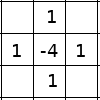
\includegraphics[scale = 0.8]{Images/Laplacian.png}
    \caption{Laplacien du pixel}
\end{figure}
Afin de trouver la solution au problème, il faut donc appliquer cette discrétisation à chaque pixel de la partie de l'image à modifier($\Omega \cup \partial \Omega$). Chaque pixel faisant intervenir ses voisins, la résolution du problème passe donc par la résolution d'un système.
En notant :
\begin{center}
 $g(x,y) = S(x+1,y) + S(x-1,y)+ S(x,y+1) + S(x,y-1) - 4\times S(x,y)$\\
 \end{center}
Résoudre $\Delta I(x,y) = \Delta S(x,y)$ sur $\Omega$ est équivalent à résoudre :\\
\begin{center}
\begin{equation*}
    \left \{
    \begin{aligned}
    I(i+1,j) + I(i-1,j)+ I(i,j+1) + I(i, j-1) - 4\times 			I(i,j)= g(i,j)\\ pour (i,j)\in \Omega \\
    I(i,j) = T(i,j) \ pour \ (i,j) \in \partial \Omega
    \end{aligned}
    \right.
\end{equation*}
\end{center}
La résolution de ce système de taille $M\times N $ permettra de trouver la nouvelle image I, et donc de résoudre numériquement l'équation de Poisson avec conditions aux bords de Dirichlet. Voici le système obtenu : 
\begin{equation}
\left\{
\begin{aligned}
I(1,1) = T(1,1)\\
I(3,2)+I(1,2)+ I(2,3)+I(2,1)-4I(2,2) =g(2,2) \\
I(3,3)+I(1,3)+ I(2,4)+I(2,2)-4I(2,3) =g(2,3)             \\
... \\
I(M,N-1)+I(M-2,N-1)+ I(M-1,N)+I(M-1,N-2)-4I(M-1,N-1) =g(M-1,N-1)\\
I(M, N) = T(M, N)
\end{aligned}
\right.
\end{equation}
\subsubsection{Résolution du système}
Afin de résoudre ce système, il est plus facile de l'écrire sous forme matricielle. Il faut maintenant trouver la solution du problème suivant : 
\begin{center}
 AI = b 
\end{center}
Si la matrice est inversible, alors la solution est évidente, et elle vaut : 
\begin{center}
$I = A^{-1}\times b$
\end{center} 
Avec : 
\begin{itemize}
\item A, une matrice carrée de taille ($M\times N$, $M\times N$)
\item I, un vecteur colonne de taille ($M\times N$,1)
\item b, un vecteur colonne de taille ($M\times N$,1)
\end{itemize}
Voici donc à quoi ressemble le système que nous souhaitons résoudre :\newline
La matrice A est une matrice par bloc. Pour la remplir, commençons par écrire l'image sous forme d'un vecteur colonne. Dans l'exemple ci-dessous nous voyons bien qu'afin de remplir les lignes de A correspondant au pixel se situant à l'intérieur du domaine, il nous faut la connaissance des voisins de celui-ci.
\begin{figure}[!h]
\centering
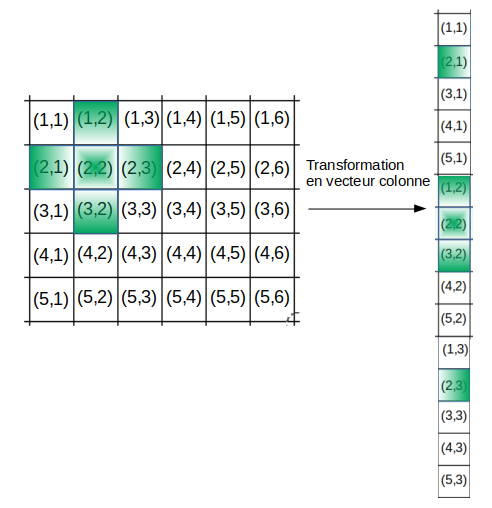
\includegraphics[scale=0.5]{Images/laplacienIJ.png}
\caption{Transformation en un vecteur colonne}
\end{figure}
Ainsi, le calcul du Laplacien du pixel (2,2) nécessite les pixels U, D, R et L. Il faut donc ajouter les coefficients correspondant dans A. Grâce au vecteur colonne obtenu, il est évident que la ligne de la matrice correspondant au pixel (i,j) à l'intérieur du domaine sera remplie de la manière  suivante : 
\begin{center}
\begin{equation}
\left.
\begin{aligned}
\begin{pmatrix}
	1 & 0 & ... &  1 &-4 & 1 & 0 & ... & 1 & 0... \\
\end{pmatrix}
\end{aligned}
\right.
\end{equation}
\end{center}
Si l'image est de taille ($M\times N$) alors : 
\begin{itemize}
\item Le coefficient (i, j-1) dans la matrice correspondant au pixel U de l'image
\item Le coefficient (i,j+1) correspondant au pixel D
\item Le coefficient (i,j+M) correspondant au pixel R
\item Le coefficient (i,j-M) correspondant au pixel L
\end{itemize}

Les blocs de la matrice correspondant aux pixels situés sur le bords du domaine seront remplis de la façon suivante : 
\begin{center}
\begin{equation}
\left.
\begin{aligned}
\begin{pmatrix}
	1 & 0& 0 & ...& 0 & 0 & 0...&0& ... & 0\\
	0 & 1 & 0 & 0 & ... & 0 &0 &0&....&0\\
	0 & 0 & 1 & 0 & 0&... &0 &0 &0&...\\
	&...\\
	0 & 0 &... &0 &0 &0 &0...& 0& 0 & 1\\
\end{pmatrix}
\end{aligned}
\right.
\end{equation}
\end{center}
Le vecteur b contient les Laplaciens des pixels à l'intérieur de $\Omega$ et les valeurs des pixels de T en dehors du domaine. 
Les valeurs des pixels de S étant connus, il est facile de calculer son Laplacien en utilisant les discrétisations vues ci-dessus. Ainsi : 
\begin{equation*}
b(i) = 
\left\{
\begin{aligned}
T(i,j) \ si \ I (i,j) \notin \Omega\\
g(i,j) \ si \ I( i,j) \in \Omega
\end{aligned}
\right.
\end{equation*}

En inversant la matrice, la solution I obtenue est un vecteur : 
\begin{center}
\begin{equation*}
\left.
\begin{aligned}
\begin{pmatrix}
I(1,1)\\
I(2,1)\\
...\\
I(1,2)\\
I(2,2)\\
....\\
I(M, N)
\end{pmatrix}
\end{aligned}
\right.
\end{equation*}
\end{center}
Afin de trouver l'image finale, il est donc important de reconstruire une matrice de taille $M\times N$ à partir de ce vecteur. 

\subsection{Exemple}
Considérons l'image S ci-contre, que nous souhaitons coller. 
\begin{figure}[!htb]
   \begin{minipage}{0.5\textwidth}
     \centering
     
\includegraphics[width = 100pt]{Images/square.png}
     \caption{Images à coller}
      \end{minipage}\hfill
   \begin{minipage}{0.5\textwidth}
     \centering
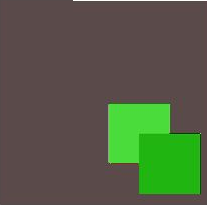
\includegraphics[width = 100pt]{Images/targer.png}
\caption{Image de fond}
      \end{minipage}\hfill
\end{figure}
Nous souhaitons ici coller les deux carrés rouges sur une image que nous nommerons T.  

\begin{figure}[!htb]
   \begin{minipage}{0.5\textwidth}
     \centering
     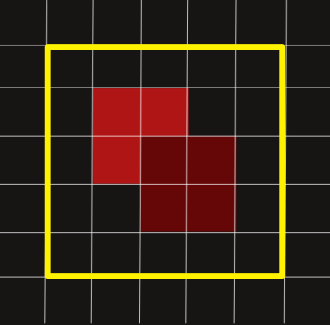
\includegraphics[width = 100pt]{Images/carre_selection.png}
\caption{Sélection à coller}
      \end{minipage}\hfill
         \begin{minipage}{0.5\textwidth}
     \centering
     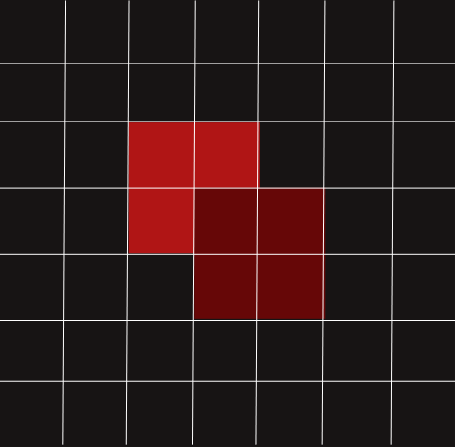
\includegraphics[width = 100pt]{Images/pix.png}
\caption{Vue grille pixel}
      \end{minipage}\hfill
      \end{figure}
\newpage

Notons $\Omega$, l'intérieur de la zone encadrée par la ligne verte, et $\partial \Omega$ les pixels appartenant à $Jaune \backslash \Omega$


\paragraph{Construction du système}
\begin{center}
\begin{equation}
\left\{
\begin{aligned}
I_{1,1} = T_{1,1}\\
...\\
I_{5,1} = T_{5,1}\\
I_{1,2} = T_{1,2}\\
\Delta I_{2,2} = \Delta S_{2,2}\\
\Delta I_{3,2} = \Delta S_{3,2}\\
\Delta I_{4,2} = \Delta S_{4,2}\\
...\\
\end{aligned}
\right.
\end{equation}
\end{center}
Avec $\Delta I(i,j) = U+D+L+R-4I(i,j)$.\\
En écrivant ce système sous forme matricielle, la matrice A est la matrice $25\times 25$ ci-dessous :  

\begin{figure}[!htb]
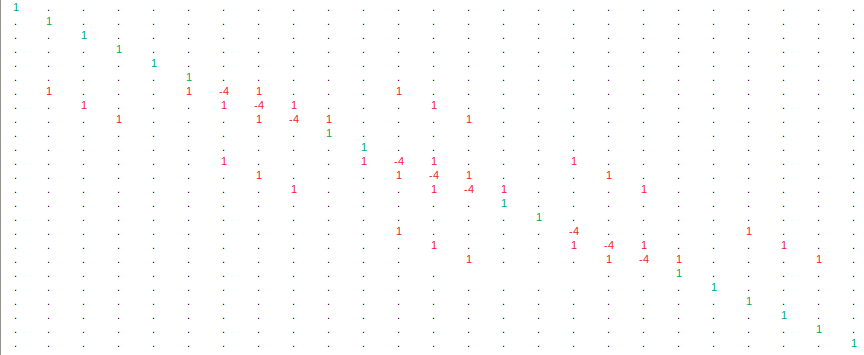
\includegraphics[scale=0.5]{Images/matrice.png}
\caption{Matrice du système}
\end{figure}
\begin{equation}
I = 
\begin{pmatrix}
I(1,1)\\
I(2,1)\\
...\\
I(5,1)\\
...\\
I(1,3)\\
...\\
I(5,3)\\
...\\
I(5,5)\\
\end{pmatrix}
b = 
\begin{pmatrix}
T(1,1)\\
...\\
\Delta S(2,2)\\
...\\
T(5,2)\\
\Delta S(1,3)\\
...\\
T(5,3)\\
\Delta S(2,4)\\
...\\
\Delta S(4,4)\\
T(5,4)\\
...\\
T(5,5)\\
\end{pmatrix}
\end{equation}
La solution de ce système existe bien. En effet, A étant carrée, de taille $\left(M\times N, M \times N\right)$. Elle est aussi toujours remplie de la même manière ('par blocs'). Ses colonnes étant linéairement indépendantes, elle est donc inversible.\\
La solution I, s'écrit sous la forme
\begin{center}
$I = A^{-1}b$.
\end{center} 
\begin{figure}[!h]
    \centering
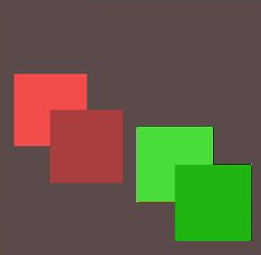
\includegraphics[width = 120pt]{Images/result.png}
\caption{Résultat obtenu}\hfill
\end{figure} 
Nous ajouterons dans la section suivante les résultats obtenus à l'aide de cette méthode. \\ Celle-ci fonctionne très bien mais le temps de calcul peut devenir très long. En effet, cette méthode demande une inversion matricielle et donc un temps de calcul relativement long sur de "très" grands systèmes, donc de très grandes sélections. Nous allons maintenant voir une seconde méthode, plus rapide sur de grandes sélections, en nous plaçant dans le domaine de Fourier.

